\documentclass[11pt]{standalone}
\usepackage[usenames]{color} %used for font color
\usepackage{amssymb} %maths
\usepackage{amsmath} %maths

\usepackage[no-math]{fontspec}
\usepackage{unicode-math}
\setmainfont{Lato}
\setmathfont{Stix Two Math}

\usepackage{pgf,xcolor}
\definecolor{itwm_blue_04}{HTML}{005A94}
\definecolor{itwm_red}{HTML}{C00000}
\definecolor{itwm_yellow}{HTML}{FFEC7F}

\usepackage{tikz}
\usetikzlibrary{shapes.misc, shadows, decorations}
\usetikzlibrary{decorations.pathreplacing,calligraphy}
\usetikzlibrary{positioning, arrows}
\usetikzlibrary{backgrounds}
\usetikzlibrary{calc}
\usepackage{pgfplots}
\pgfplotsset{compat=newest}
\usepgfplotslibrary{fillbetween}
\usepackage{tikzpagenodes}
\usetikzlibrary{patterns}


\begin{document}
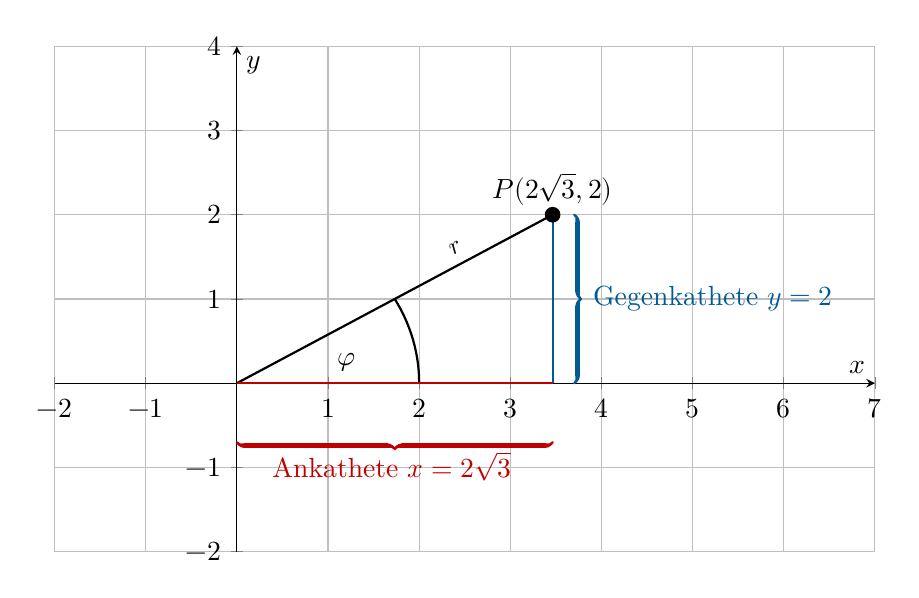
\begin{tikzpicture}
\begin{axis}[
    domain=-2:7,
    axis lines = center,
    xlabel = {$x$},
    ylabel = {$y$},
    height=8cm, width=12cm, 
    xmin=-2, xmax=7, ymin=-2, ymax=4,
    xtick={-2,-1,...,7},
    ytick={-2,-1,...,4},
    grid = both
]
\draw[itwm_blue_04, thick] (3.4641,0) -- (3.4641,2) {};
\draw[thick] (0,0) -- (3.4641,2) {};
\draw[thick] (2,0) arc[start angle=0, end angle=30, radius=2];
\node at (1.2,0.25) {$\varphi $};
% Calligraphic brace
\draw [pen colour={itwm_blue_04}, decorate,
    decoration = {calligraphic brace, mirror}, ultra thick] (3.7,0) --  (3.7,2);
\node[right, itwm_blue_04] at (3.8,1) {Gegenkathete $y = 2$};
%
\draw[itwm_red, thick] (0,0) -- (3.4641,0) {};
\draw [pen colour = {itwm_red}, decorate,
    decoration = {calligraphic brace, mirror}, ultra thick, itwm_red] (0,-0.7) --  (3.4641,-0.7);
\node[below, itwm_red] at (1.7,-0.7) {Ankathete $x = 2\sqrt{3}$};
\node[fill, black, circle, inner sep=-2] at (3.4641,2) {};
\node[above] at (3.4641,2) (point) {$P(2\sqrt{3},2)$};
\node[font=\fontsize{9}{0}\selectfont, rotate=30] at (2.4,1.6) {$r$};
\end{axis}
\end{tikzpicture}
\end{document}

